\section{Adam Szlósarczyk}

I added a photo of a Bengal tiger (see Figure \ref{fig:tiger})

\begin{figure}[htbp]
    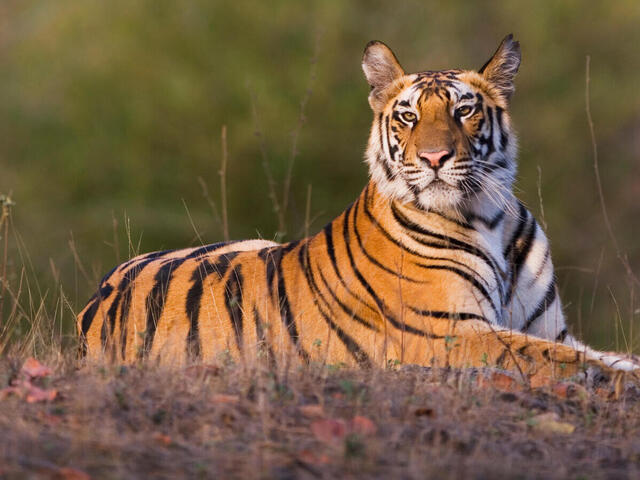
\includegraphics[width=\linewidth]{pictures/tiger.jpg}
    \caption{17 months old Bengal tiger cub (male) resting in open area early morning, dry season.}
    \label{fig:tiger}
\end{figure}

\newpage

Table \ref{tab:programming_languages_table} shows the list of the 5 most popular programming languages

\begin{table}[htbp]
\centering
\begin{tabular}{|c|c|c|}
\hline
\rowcolor[HTML]{C0C0C0} 
\textbf{Programming language} & \textbf{Ratings} & \textbf{Change} \\ \hline
Python                        & 14.82\%          & -2.25\%         \\ \hline
C                             & 12.08\%          & -3.13\%         \\ \hline
C++                           & 10.67\%          & +0.74\%         \\ \hline
Java                          & 8.92\%           & -3.92\%         \\ \hline
C\#                           & 7.71\%           & +3.29\%         \\ \hline
\end{tabular}
\label{tab:programming_languages_table}
\caption{5 most popular programming languages as of Oct 2023}
\end{table}

Given a general quadratic equation \ref{eq_quadratic} of the form
\begin{equation} \label{eq_quadratic}
ax^2 + bx + c = 0
\end{equation}
with x representing an unknown, with a, b and c representing constants, and with a $\neq$ 0, the quadratic formula is:
\begin{equation}
x = \frac{-b \pm \sqrt{b^2 - 4ac}}{2a}
\end{equation}

Here is also a worth seeing equation: \[V=\frac{1}{3}\pi r^2h\]

It is used to calculate the volume of a cone

And another one: 
$ (\sin x)^2 + (\cos x)^2 = 1 $

\bigskip

Ordered list of the most populated countries in the world
\begin{enumerate}
    \item India
    \item China
    \item United States
    \item Indonesia
    \item Pakistan
\end{enumerate}

\newpage

Continents of the World:
\begin{itemize}
    \item Asia
    \item Africa
    \item Europe
    \item North America
    \item South America
    \item Australia/Oceania
    \item[-] Antarctica
\end{itemize}

\hspace{\parindent}\textbf{Europe} is a \textbf{continent} comprising the westernmost peninsulas of Eurasia, located entirely in the \underline{Northern Hemisphere} and mostly in the \underline{Eastern} \underline{Hemisphere}. It shares the continental landmass of Afro-Eurasia with both Africa and Asia. It is bordered by the Arctic Ocean to the north, the Atlantic Ocean to the west, the Mediterranean Sea to the south, and Asia to the east. \textbf{Europe} is commonly considered to be separated from Asia by the watershed of the \textit{Ural Mountains}, \textit{the Ural River}, \textit{the Caspian Sea}, \textit{the Greater Caucasus}, \textit{the Black Sea} and \textit{the waterways of the Turkish straits}.

\hspace{\parindent}\textbf{Europe} covers about 10.18 million km2 (3.93 million sq mi), or 2\% of Earth's surface (6.8\% of land area), making it the second-smallest continent (using the seven-continent model). Politically, \textbf{Europe} is divided into about fifty sovereign states, of which Russia is the largest and most populous, \emph{spanning 39\% of the continent and comprising 15\% of its population.} \textbf{Europe} had a total population of about \underline{745 million} (about 10\% of the world population) in 2021; the third-largest after Asia and Africa. The European climate is largely affected by warm Atlantic currents that temper winters and summers on much of the continent, even at latitudes along which the climate in Asia and North America is severe. Further from the sea, seasonal differences are more noticeable than close to the coast.

\newpage